\documentclass[a4paper,11pt]{report}

% Packages
\usepackage[utf8]{inputenc}
\usepackage[T1]{fontenc}
\usepackage{geometry}
\usepackage{graphicx}
\usepackage{hyperref}
\usepackage{titlesec}
\usepackage{parskip}

% Geometry setup
\geometry{
    top=2.5cm,
    bottom=2.5cm,
    left=2.5cm,
    right=2.5cm
}

% Hyperref setup
\hypersetup{
    colorlinks=true,
    linkcolor=blue,
    filecolor=magenta,      
    urlcolor=cyan,
    pdftitle={Software Requirements Specification},
    pdfpagemode=FullScreen,
}

% Title Page Data
\title{
    \textbf{Software Requirements Specification} \\
    \vspace{1cm}
    \large \textbf{MEA-V2G / FreeV2G} \\
    \vspace{0.5cm}
    \large Reference Implementation for ISO 15118 EV/EVSE
}
\author{Development Team}
\date{\today}

\begin{document}

\maketitle
\tableofcontents
\newpage

\chapter{Introduction}

\section{Purpose}
The purpose of this document is to define the software requirements for the MEA-V2G (FreeV2G) project. This system serves as a reference implementation for controlling the 8devices WHITE-beet-EI (EVSE) and WHITE-beet-PI (EV) ISO 15118 modules using an Ethernet host control interface (HCI).

\section{Scope}
The MEA-V2G software encompasses:
\begin{itemize}
    \item Parsing of the protocol used to communicate with the WHITE-beet modules.
    \item Simulation of EVSE and EV behaviors.
    \item Handling of charging parameters (Voltage, Current, Power).
    \item Implementation of basic Control Pilot (CP) and SLAC sequences.
    \item High-level V2G communication management.
\end{itemize}

\section{Definitions and Acronyms}
\begin{description}
    \item[EV] Electric Vehicle
    \item[EVSE] Electric Vehicle Supply Equipment (Charging Station)
    \item[HCI] Host Control Interface
    \item[SLAC] Signal Level Attenuation Characterization
    \item[V2G] Vehicle-to-Grid
    \item[PNC] Plug \& Charge
    \item[EIM] External Identification Means
\end{description}

\chapter{Overall Description}

\section{Product Perspective}
The software interacts directly with the WHITE-beet hardware modules via Ethernet or SPI. It acts as the "Host" controller, managing the logic while the WHITE-beet module handles the low-level PLC (Power Line Communication) and ISO 15118 framing.

\section{System Functions}
The system enables the following core functions:
\begin{enumerate}
    \item \textbf{Control Pilot (CP) implementation}: Detects EV plugin and manages duty cycles.
    \item \textbf{SLAC}: Automates the matching process between EV and EVSE at the physical layer.
    \item \textbf{V2G Session Management}: Handles Service Discovery, Parameter Discovery, and Authorization.
    \item \textbf{Charging Loop}: Monitoring and control of the active energy transfer.
\end{enumerate}

\section{Use Case Diagram}
The following diagram illustrates the primary actors and use cases for the MEA-V2G system.

\begin{figure}[h]
    \centering
    % In execution, make sure use_case_diagram.pdf exists in the same build dir or use correct path
    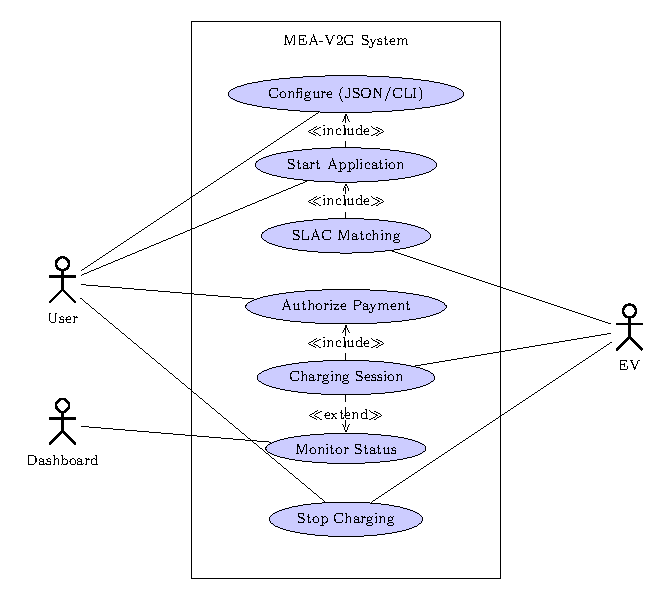
\includegraphics[width=0.9\textwidth]{use_case_diagram.pdf} 
    \caption{MEA-V2G High-Level Use Case Diagram}
    \label{fig:usecase}
\end{figure}

\section{System Architecture}
The system obeys a modular object-oriented architecture. The core logic handles the state machines for EV and EVSE, while the `Whitebeet` class abstracts the hardware communication.

\begin{figure}[h]
    \centering
    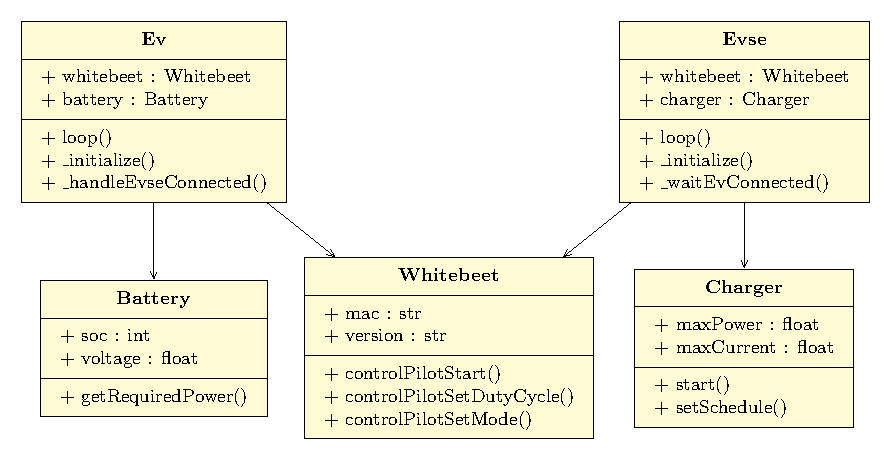
\includegraphics[width=\textwidth]{class_diagram.pdf}
    \caption{MEA-V2G Simplified Class Diagram}
    \label{fig:classdiagram}
\end{figure}

\section{Core Components}
The system comprises the following key software components:

\subsection{Whitebeet Component}
The \texttt{Whitebeet} class serves as the Hardware Abstraction Layer (HAL). It manages the low-level communication with the physical ISO 15118 module via Ethernet or SPI.
\begin{itemize}
    \item \textbf{Packet Framing}: Handles the encapsulation of Host Control Interface (HCI) commands.
    \item \textbf{Event Dispatching}: Receives raw data from the hardware and dispatches events (e.g., \texttt{EV\_CONNECTED}, \texttt{V2G\_MESSAGE}) to the higher-level logic.
    \item \textbf{Service Management}: Exposes methods to control Control Pilot (CP) state, SLAC, and V2G messaging.
\end{itemize}

\subsection{EV Component}
The \texttt{EV} class is the central controller for the client side. It orchestrates the charging session from the vehicle's perspective.
\begin{itemize}
    \item \textbf{State Machine}: Implements the ISO 15118 client flow (Session Setup $\rightarrow$ Charge Parameter Discovery $\rightarrow$ Power Delivery).
    \item \textbf{Hardware Aggregation}: Owning instance of \texttt{Whitebeet} (for comms) and \texttt{Battery} (for energy simulation).
\end{itemize}

\subsection{EVSE Component}
The \texttt{EVSE} class is the central controller for the station side. It manages the server-side logic and power delivery authorization.
\begin{itemize}
    \item \textbf{State Machine}: Implements the ISO 15118 server flow, including Service Discovery and Plug \& Charge authorization.
    \item \textbf{Hardware Aggregation}: Owning instance of \texttt{Whitebeet} (for comms) and \texttt{Charger} (for power delivery simulation).
    \item \textbf{Scheduling}: Manages SASchedules based on configuration.
\end{itemize}

\section{Charger Component}
The \texttt{Charger} class performs a physical simulation of the power electronics, ensuring realistic behavior during the charging session. Its key functions include:
\begin{itemize}
    \item \textbf{Output Ramping}: Instead of instantaneous jumps, the charger simulates the physical "slewing" of voltage and current over time. It uses defined $\Delta U$ and $\Delta I$ rates to ramp the output toward the target setpoint.
    \item \textbf{Limit Enforcement}: It strictly enforces hard safety limits for the system (e.g., \texttt{evse\_max\_current}, \texttt{evse\_max\_power}), protecting the modeled hardware.
    \item \textbf{Setpoint Control}: The EV provides dynamic target values (\textit{Target Voltage}, \textit{Target Current}), which the charger attempts to follow within its safety constraints.
    \item \textbf{Fault Detection}: The class includes methods like \texttt{isVoltageLimitExceeded()} and \texttt{isPowerLimitExceeded()} to trigger immediate session termination if operating conditions are violated.
\end{itemize}

\section{Battery Component}
The \texttt{Battery} class provides a logical model of the EV's energy storage, managing State of Charge (SOC) and physical limits.
\begin{itemize}
    \item \textbf{Energy Tracking}: Maintains the battery capacity (Wh) and current energy level. SOC is dynamically calculated as $\frac{\textit{Current Level}}{\textit{Capacity}} \times 100$.
    \item \textbf{Charging Process}: The \texttt{tickSimulation()} method accumulates energy over time intervals based on the instantaneous input voltage and current ($E = V \times I \times \Delta t$).
    \item \textbf{Configurable Limits}: Supports defining maximum Voltage, Current, and Power constraints specific to the chosen Energy Transfer Mode (AC vs. DC).
    \item \textbf{Status Reporting}: Continuously updates the SOC and charging status ('is\_full', 'is\_charging'), which are reported back to the EVSE via ISO 15118 messages.
\end{itemize}

\chapter{Specific Requirements}

\section{External Interfaces}

\subsection{Communication Interfaces}
\begin{itemize}
    \item \textbf{Ethernet}: Main control interface for sending HCI commands and receiving notifications.
    \item \textbf{SPI}: Alternative control interface (e.g., for Raspberry Pi integration).
\end{itemize}

\subsection{User Interfaces}
\begin{itemize}
    \item \textbf{CLI (Command Line Interface)}: Primary mode of operation. Outputs session logs and accepts interactive input (e.g., authorization "yes/no").
    \item \textbf{GUI}: A graphical launcher (`gui\_launcher.py`) provided for configuration and startup.
    \item \textbf{API}: A REST API (default port 5000) for real-time status monitoring (e.g., for Grafana dashboards).
\end{itemize}

\section{Functional Requirements}

\subsection{FR-01: Protocol Negotiation}
The system shall support negotiation of ISO 15118 protocol versions.
\begin{itemize}
    \item The EVSE shall advertise supported protocols.
    \item The EV shall select a mutually supported protocol (e.g., DIN SPEC 70121 or ISO 15118-2).
\end{itemize}

\subsection{FR-02: Authorization}
The system shall support multiple authorization modes:
\begin{itemize}
    \item \textbf{EIM (External Identification Means)}: Manual authorization via console input.
    \item \textbf{PnC (Plug \& Charge)}: Automated certificate-based authorization.
\end{itemize}

\subsection{FR-03: Charging Control}
During the charging loop, the system shall:
\begin{itemize}
    \item Exchange charging parameters (SOC, Target Voltage, Target Current).
    \item Terminate the session upon "Stop Charging" request from either side.
\end{itemize}

\section{Communication Flow}
The following sequence diagram depicts the simplified ISO 15118 charging loop interaction between the EV and EVSE, which is the core logical flow of the application.

\begin{figure}[h]
    \centering
    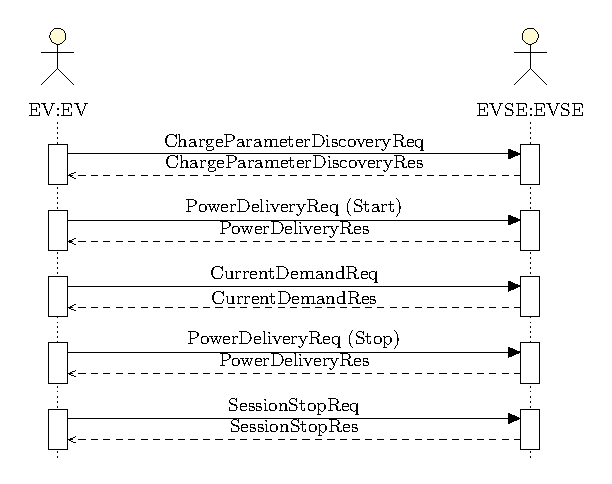
\includegraphics[width=0.8\textwidth]{sequence_diagram.pdf}
    \caption{ISO 15118 Charging Loop Sequence}
    \label{fig:sequenceinteraction}
\end{figure}

\section{EV State Machine}
The EV internal logic follows a distinct state machine to manage the charging session lifecycle, as observed in the implementation.

\begin{description}
    \item[Init] Initial state where the EV controller is started and hardware interfaces (SPI/Ethernet) are initialized.
    \item[SessionStarted] The V2G session has been established. The EV has successfully matched with the EVSE via SLAC.
    \item[CableCheck] The EV waits for the EVSE to perform the cable check (isolation test) to ensure safety.
    \item[PreCharging] Pre-charge phase where the EV matches its battery voltage to the DC bus voltage.
    \item[Charging] The main state where energy transfer occurs. The EV sends \textit{CurrentDemand} requests in a loop.
    \item[ChargingStopped] The session is terminated, either normally (target SOC reached) or due to an error.
\end{description}

\begin{figure}[h]
    \centering
    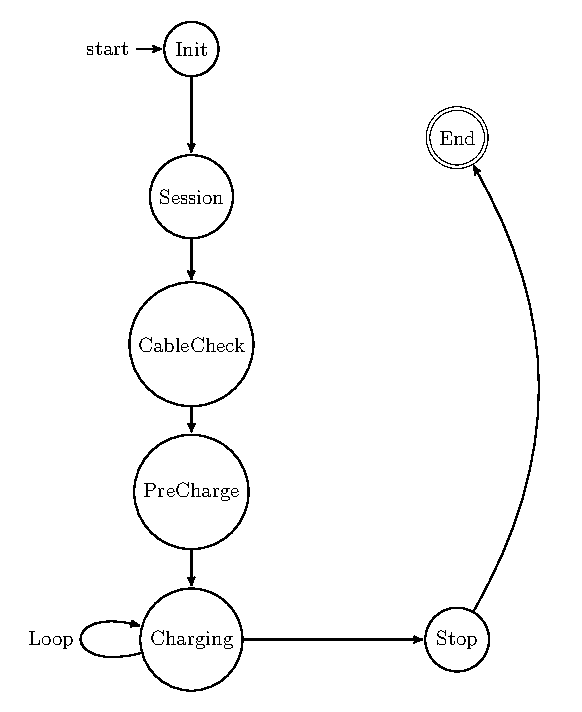
\includegraphics[width=0.6\textwidth]{state_diagram.pdf}
    \caption{EV State Machine}
    \label{fig:statediagram}
\end{figure}

\section{EVSE State Machine}
The EVSE logic complements the EV, acting as the server component that handles session setup, authorization, and power delivery control.

\begin{description}
    \item[Init] Initialization of the Whitebeet module services (CP, SLAC, V2G).
    \item[Wait] The EVSE waits for an EV to physically plug in (Control Pilot State B).
    \item[SLAC] Signal Level Attenuation Characterization process to pair the EV and EVSE.
    \item[Session] High-level communication session established; protocol negotiation occurs.
    \item[Authorization] Verifying if the EV is authorized to charge (via EIM or Plug \& Charge).
    \item[Params] Exchanging charge parameter limits (Maximum Voltage, Current, Power limits).
    \item[Cable] Performing cable isolation check to ensure no faults exist.
    \item[PreCharge] Adjusting DC output voltage to match the EV's reported battery voltage.
    \item[Charge] Active energy transfer loop responding to the EV's current demand.
    \item[Stop] Session termination and welding detection sequence.
\end{description}

\begin{figure}[h]
    \centering
    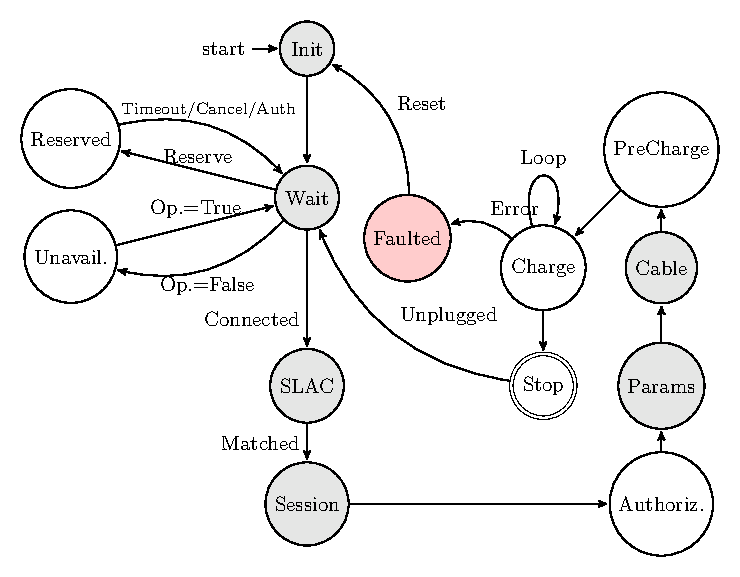
\includegraphics[width=0.7\textwidth]{evse_state_diagram.pdf}
    \caption{EVSE State Machine}
    \label{fig:evsestatediagram}
\end{figure}

\section{State Synchronization}
The charging process relies on the tight synchronization between the EV and EVSE states. Figure \ref{fig:staterelation} illustrates the parallel state progression and key synchronization points.

\begin{description}
    \item[Discovery] Control Pilot signal detection (State A $\rightarrow$ B).
    \item[Setup] SLAC matching and V2G Session Setup.
    \item[Safety] Both sides must confirm safety parameters during Cable Check.
    \item[Sync] Voltage levels must be synchronized during Pre-Charge before the contactors close.
    \item[Power] The Charging Loop is a lock-step process where the EV requests and the EVSE delivers.
    \item[Term] Coordinated shutdown to ensure contactors open safely (Welding Detection).
\end{description}

\begin{figure}[h]
    \centering
    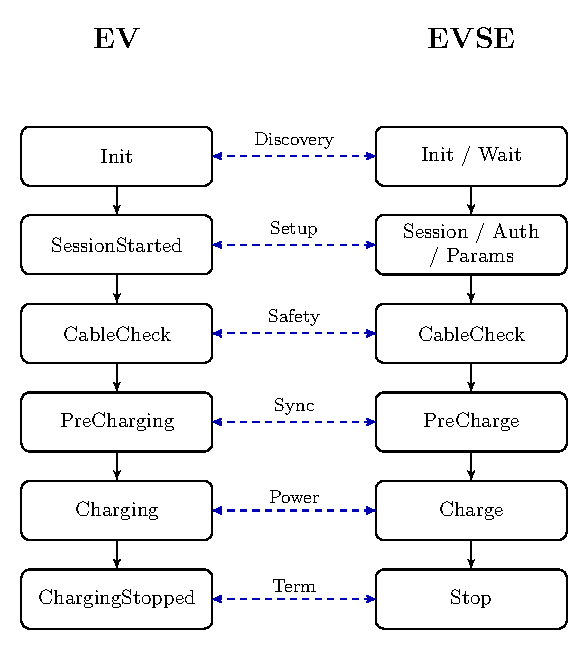
\includegraphics[width=0.8\textwidth]{states_relation_diagram.pdf}
    \caption{EV-EVSE State Synchronization}
    \label{fig:staterelation}
\end{figure}

\chapter{Configuration and Deployment}

\section{Command Line Interface (CLI)}
The system is launched via \texttt{Application.py} with several arguments to define its operating mode:

\begin{itemize}
    \item \texttt{-r, --role}: Specifies the mode of operation (\texttt{EV} or \texttt{EVSE}).
    \item \texttt{-i, --interface}: Defines the network interface connected to the Whitebeet module (e.g., \texttt{eth0}).
    \item \texttt{-c, --config}: Path to the EV configuration file (default: \texttt{ev.json}).
    \item \texttt{-ec, --evse-config}: Path to the EVSE configuration file (default: \texttt{evse.json}).
    \item \texttt{--auto}: (EVSE only) Enables automatic authorization for Plug \& Charge.
    \item \texttt{--api-port}: Sets the port for the REST API status monitor.
\end{itemize}

\section{JSON Configuration}
Behavioral parameters are externalized in JSON files to allow run-time customization without code changes.

\subsection{EV Configuration (ev.json)}
Defines the characteristics of the Electric Vehicle:
\begin{itemize}
    \item \textbf{ev}: Supported protocols (ISO 15118-2, DIN), payment methods (EIM, PnC), and energy transfer modes.
    \item \textbf{battery}: Physical parameters including capacity, maximum voltage/current, and initial SOC.
\end{itemize}

\subsection{EVSE Configuration (evse.json)}
Defines the characteristics of the Charging Station:
\begin{itemize}
    \item \textbf{charger}: Output limits (Max Voltage/Current/Power) and slew rates ($\Delta V, \Delta I$) for the simulation.
    \item \textbf{schedule}: Defines power delivery schedules (SASchedules) sent to the EV during the Charge Parameter Discovery phase.
\end{itemize}

\end{document}
